%!TEX root = edance.tex
%%%%%%%%%%%%%%%%
%  CHAPTER 17  %
%%%%%%%%%%%%%%%%
\chapter{Op-Amp Feedback and Frequency Response}
\label{ch:ch17_opamps_fb}
\graphicspath{{./figs_opamps_fb/}}
%%%%%%%%%%%%%%%%%%%%%%%%%%%%%%%%%%%%%%%%%%%%%%%%%%%%%%%%%%%%%%%%%%%%%%%%%%%%%%%%%%%%%%%%
%%%%%%%%%%%%%%%%%%%%%%%%%%%%%%%%%%%%%%%%%%%%%%%%%%%%%%%%%%%%%%%%%%%%%%%%%%%%%%%%%%%%%%%%
%                                   SECTION 17.1                                       %
%%%%%%%%%%%%%%%%%%%%%%%%%%%%%%%%%%%%%%%%%%%%%%%%%%%%%%%%%%%%%%%%%%%%%%%%%%%%%%%%%%%%%%%%
%%%%%%%%%%%%%%%%%%%%%%%%%%%%%%%%%%%%%%%%%%%%%%%%%%%%%%%%%%%%%%%%%%%%%%%%%%%%%%%%%%%%%%%%
\section{Chapter Preview}
In this chapter we will explore operational amplifiers (op-amps) and feedback, and in particular how feedback impacts the frequency response of operational amplifiers.  We assume some familiarity with ideal op-amps, and the ``Golden Rules" for analyzing op-amp circuits, but our goal is to learn to analyze actual op-amps, not ideal ones.  We will set the context of the chapter by reviewing feedback theory in general, and motivate why feedback is important and useful.  To analyze op-amps, we need an equivalent circuit model, something more sophisticated than the ``Golden Rules" (infinite gain, infinite input impedance), but not too complicated.   We will be inspired by a physical model based on the real inner workings of an op-amp, and armed with this model we will discuss important concepts such as the gain-bandwidth product, the unity gain frequency, and the gain-bandwidth trade offs.  We end the chapter by introducing some more advanced topics, such as feedback and stability.  We don't do justice to this topic, our goal for now is to make the reader aware of the issues without understanding the details of how the issue is addressed.  This topic should be pursued in a more advanced course on analog circuit design. 
%%%%%%%%%%%%%%%%%%%%%%%%%%%%%%%%%%%%%%%%%%%%%%%%%%%%%%%%%%%%%%%%%%%%%%%%%%%%%%%%%%%%%%%%
%%%%%%%%%%%%%%%%%%%%%%%%%%%%%%%%%%%%%%%%%%%%%%%%%%%%%%%%%%%%%%%%%%%%%%%%%%%%%%%%%%%%%%%%
%                                   SECTION 17.2                                       %
%%%%%%%%%%%%%%%%%%%%%%%%%%%%%%%%%%%%%%%%%%%%%%%%%%%%%%%%%%%%%%%%%%%%%%%%%%%%%%%%%%%%%%%%
%%%%%%%%%%%%%%%%%%%%%%%%%%%%%%%%%%%%%%%%%%%%%%%%%%%%%%%%%%%%%%%%%%%%%%%%%%%%%%%%%%%%%%%%
\section{Introduction to Feedback}
%%%%%%%%%%%%%%%%%%%%%%%%%%%%%%%%%%%%%%%%%%%%
%             SUBSECTION 17.2.1            %
%%%%%%%%%%%%%%%%%%%%%%%%%%%%%%%%%%%%%%%%%%%%
\subsection{Feedback Control}
%%%%%%%%%%%%%%%%%%%%%%%%%%%%%%%%%%%%%%%%%%%%
%                 FIGURE                   %
%%%%%%%%%%%%%%%%%%%%%%%%%%%%%%%%%%%%%%%%%%%%
\begin{figure}[tb]
\centering
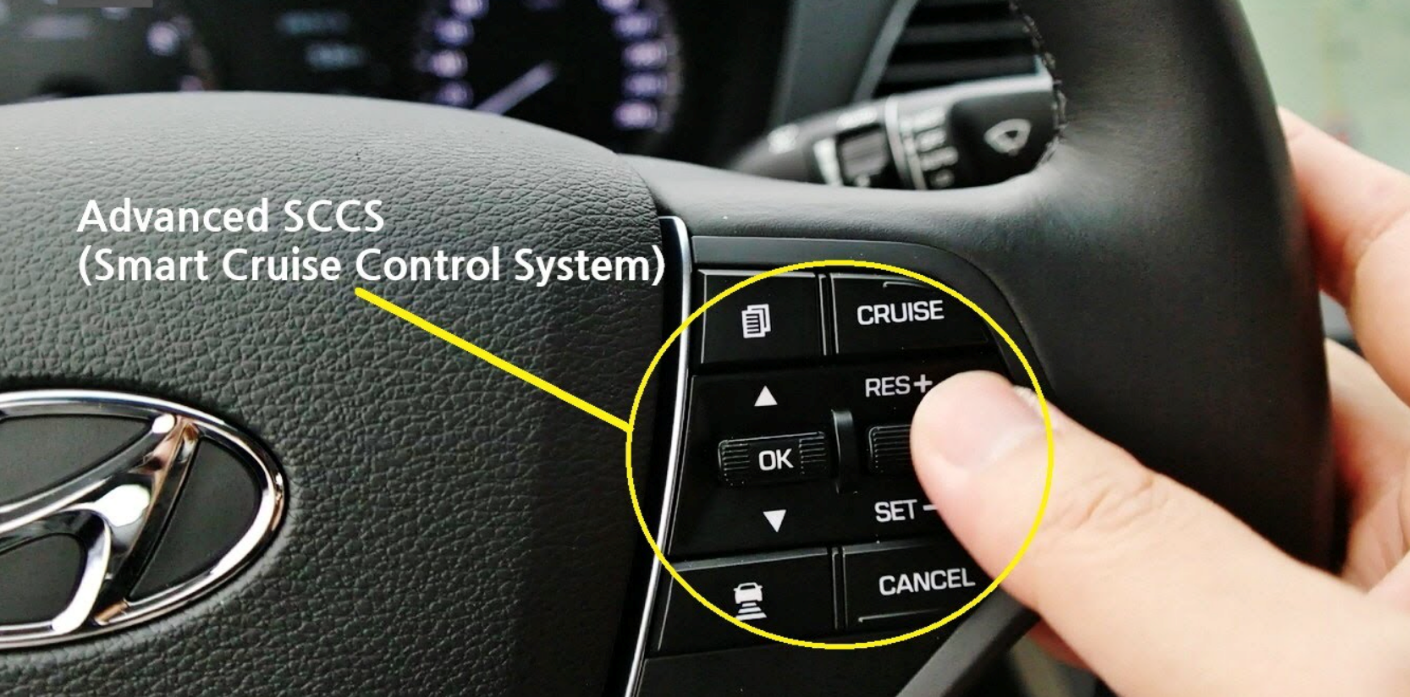
\includegraphics[width=.5\columnwidth]{image_0.png}
\caption{The cruise control system in an automobile is an example of a feedback control system.} \label{fig:image_0.png}
\end{figure}
%%%%%%%%%%%%%%%%%%%%%%%%%
\textbf{Feedback}\index{Feedback} is a universal way to design a system that is characterized by a lot of unknowns.  Think about the thermostat in your house, or the cruise control system in your car.  Humans also rely extensively on feedback -- everything from our endocrine system (hormones) to the very act of walking, relies on positive and negative feedback loops.  

Let's focus on the speed control or cruise control system in particular (see \emph{Fig.~\ref{fig:image_0.png}}).  The important steps to run the feedback loop can be summarized as follows:
    \begin{itemize}
        \item We input the desired speed of car ($v_{des}$)
        \item The car measure the actual speed of car ($v_{car}$)
        \item The control system generates an error signal, which is the difference between the current speed and the desired speed ($v_{err} = v_{des} - v_{car}$).
    \end{itemize}

Based on $v_{err}$, the system takes action.  For example, adjusting the car speed (accelerate or decelerate) based on the signal $K_p v_{err}$ where $K_p$ is a proportionality constant.\footnote{More complicated control schemes can also take action based on not only the error signal, but also based on the integral or derivative of the error signal, altering the dynamics of the system.  These controllers are called ``PID" controllers because they respond to changes \emph{P}roportional to the \emph{I}ntegral or \emph{D}erivative of the error system.}

What is important to take away from the above example is that the control system is somewhat blind to the details of how the car or engine works, it just tries to set the speed by adjusting the current speed.  This is a powerful model for designing systems, because it allows us to abstract away all the details and focus on the problem at hand.  Your thermostat in your house is a perfect example of this as it has no knowledge about the size of your house, the number of windows, the presence of insulation in the walls, etc.  It simply turns on the heater when the temperature is lower than desired, and keeps the heat on until the desired temperature has been obtained.  
%%%%%%%%%%%%%%%%%%%%%%%%%%%%%%%%%%%%%%%%%%%%
%             SUBSECTION 17.2.2            %
%%%%%%%%%%%%%%%%%%%%%%%%%%%%%%%%%%%%%%%%%%%%
\subsection{Negative Feedback Block Diagram}
%%%%%%%%%%%%%%%%%%%%%%%%%%%%%%%%%%%%%%%%%%%%
%                 FIGURE                   %
%%%%%%%%%%%%%%%%%%%%%%%%%%%%%%%%%%%%%%%%%%%%
\begin{figure}[tb]
\centering
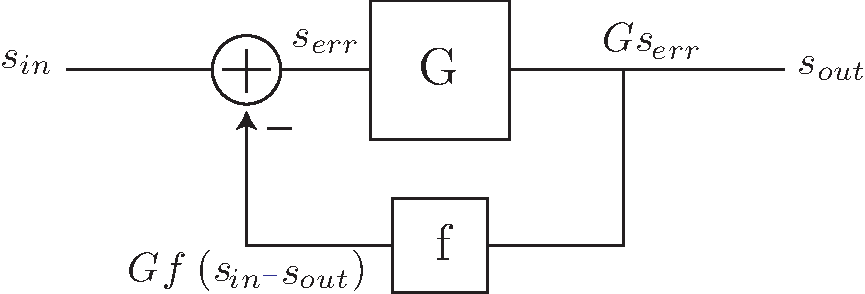
\includegraphics[scale=.7]{fbblock2}
\caption{Block diagram model of a feedback system.  $G$ is the forward gain and $f$ is the feedback factor.  The input signal $s_{in}$ is combined with a fraction of the output $f s_{out}$ and forms the error signal $s_{err}$.}
\label{fig:fbblock2}
\end{figure}
%%%%%%%%%%%%%%%%%%%%%%%%%%%%%%%%%%%%%%%%%%%%
Let's analyze a feedback system using equations.  The model for a general feedback system is shown in \emph{Fig.~\ref{fig:fbblock2}}.  This is a negative feedback system because we subtract the feedback signal from the input in order to generate the error signal.  This subtraction is represented by the (+) with the circle around it, and the (-) underneath it in the figure.

To find the transfer function, note that the error signal is a function of the input, and output after it has been fed back through the \emph{``f''} box.:
    \begin{equation}
        {s_{err}} = {s_{in}} - f \cdot {s_{out}}
    \end{equation}
and the output is the amplified error signal:
    \begin{equation}
        {s_{out}} = G \cdot {s_{err}} = G \cdot ({s_{in}} - f{s_{out}})
        \label{eq:amp_error}
    \end{equation}
\newpage
There's a bit of strangeness in \emph{Eq.~\ref{eq:amp_error}},  because the output is a function of itself.  In other words, the current output depends on the current output and the current input, which is somewhat recursive or self-referential.  From a mathematical perspective, there is nothing wrong with this equation, and we can readily solve it.  But, from an intuition perspective, we can resolve this circular reference by imagining a slight delay in the above equation:
    \begin{equation}
        {s_{out}(t)} = G \cdot {s_{err}(t) } = G \cdot ({s_{in}(t)} - f{s_{out}(t-\tau)})
    \end{equation}
In fact, this models real systems better because often there is a delay in sampling the output signal and applying it to the control system.  In electronic systems this delay is actually vanishingly small (due to the large velocity of light propagation), so we ignore it for the rest of the chapter.\footnote{There is a delay in the system due to the frequency phase response of the gain $G$, and this will be explained later on.  If the delay is not small, the system can be analyzed using Laplace Transform techniques.}  
%%%%%%%%%%%%%%%%%%%%%%%%%%%%%%%%%%%%%%%%%%%%
%              SUB-SUBSECTION              %
%%%%%%%%%%%%%%%%%%%%%%%%%%%%%%%%%%%%%%%%%%%%
\subsubsection{Closed-Loop Transfer Function}
To solve for the transfer function, we group terms involving $s_{out}$ in \emph{Eq.~\ref{eq:amp_error}}, and solve:
    \begin{align*}
        s_{out} &= G \cdot (s_{in} - f{s_{out}})\\
        &= G \cdot s_{in} - G \cdot f{s_{out}}
    \end{align*}
Moving both $s_{out}$ terms to the LHS, and factoring, we have:
    \begin{equation*}
        s_{out}(1 + Gf) = G \cdot s_{in}
    \end{equation*}
This leads to:
    \begin{equation}
        {G_{closed}} = \frac{{{s_{out}}}}{{{s_{in}}}} = \frac{G}{{1 + Gf}}
    \end{equation}
For very large gain $G$, such that $Gf \gg 1$, we have:
    \begin{equation}
        {G_{closed}} \approx \frac{G}{{Gf}} = \frac{1}{f}
        \label{eq:largegain}
    \end{equation}
This end result is very interesting because it says the transfer function does not depend on $G$, but only on the feedback!  Imagine if $G$ is an unknown or ill-defined function.  For example, if we design an amplifier, the gain will vary due to process variations, temperature, voltage variations (supply), or through aging.  All of these effects make it very difficult to build a reliable and precise amplifier without feedback.  With feedback, we can make a precise gain if we can make a well defined \textbf{feedback factor}\index{Feedback!Feedback factor} $f$.
\newpage
%%%%%%%%%%%%%%%%%%%%%%%%%%%%%%%%%%%%%%%%%%%%
%             SUBSECTION 17.2.3            %
%%%%%%%%%%%%%%%%%%%%%%%%%%%%%%%%%%%%%%%%%%%%
\subsection{Electronic Feedback}
%%%%%%%%%%%%%%%%%%%%%%%%%%%%%%%%%%%%%%%%%%%%
%                 FIGURE                   %
%%%%%%%%%%%%%%%%%%%%%%%%%%%%%%%%%%%%%%%%%%%%
\begin{figure}[tb]
\centering
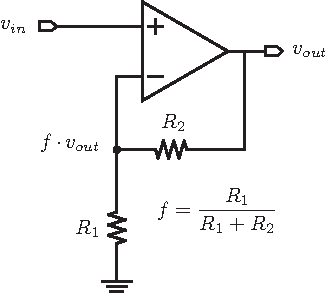
\includegraphics[scale=1]{opamp_fb}
\caption{A non-inverting amplifier is a perfect demonstration of an electronic feedback system.  The resistive divider forms the feedback network and the error signal is calculated from the op-amp differential input.}
\label{fig:opamp_fb}
\end{figure}
%%%%%%%%%%%%%%%%%%%%%%%%%%%%%%%%%%%%%%%%%%%%
We have already seen electronic feedback in op-amps, but you probably didn't think of it that way.  For example, the non-inverting amplifier shown in \emph{Fig.~\ref{fig:opamp_fb}} can be mapped to a feedback system very easily.  The resistor divider samples the output voltage, and the error signal is formed at the input of the op-amp.  The op-amp output is an amplified copy of the error signal.  A typical op-amp has a very large value of gain, making $G f$ large, and so the gain is very accurately predicated by \emph{Eq.~\ref{eq:largegain}}:
    \begin{equation}
        G \approx \frac{1}{f} = \frac{R_1 + R_2}{R_1} = 1 + \frac{R_2}{R_1}
    \end{equation}
Notice that the gain of the op-amp is immaterial as long as it's large enough.  We may now appreciate the origin of the Golden Rules.  If the gain is allowed to go to infinity, then the error signal must be zero, and the output is $0 \cdot \infty$ or $0/0$, which is undefined unless you take the limit of gain as it approaches infinity.  All practical op-amps have finite gain, so the error signal is nearly zero, and the Golden Rules are very useful.  
%%%%%%%%%%%%%%%%%%%%%%%%%%%%%%%%%%%%%%%%%%%%
%             SUBSECTION 17.2.4            %
%%%%%%%%%%%%%%%%%%%%%%%%%%%%%%%%%%%%%%%%%%%%
\subsection{History}
Feedback in electronic systems was invented by Harold Black.  He was on a ferry ride to Bell Labs (1927) thinking about how to increase the gain and improve linearity of vacuum tube amplifiers, when in a flash of genius he realized that \textit{positive} feedback can be used to boost the gain, and \textit{negative} feedback could improve the linearity (see \emph{Fig.~\ref{fig:image_1.jpg}}).
This is a good example of a ``back of the envelope" calculation (in this case a newspaper) that changed the world.  This idea came to him after tirelessly working on the problem over the course of years, trying to improve the linearity of amplifiers.  All the open-loop vacuum tube\footnote{A vacuum tube is similar to a transistor.} amplifier topologies that he tried were plagued by problems.  But the feedback amplifier proved to be a great success.
\newpage
%%%%%%%%%%%%%%%%%%%%%%%%%%%%%%%%%%%%%%%%%%%%
%                 FIGURE                   %
%%%%%%%%%%%%%%%%%%%%%%%%%%%%%%%%%%%%%%%%%%%%
\begin{figure}[t]
\centering
\begin{tabular}{cc}
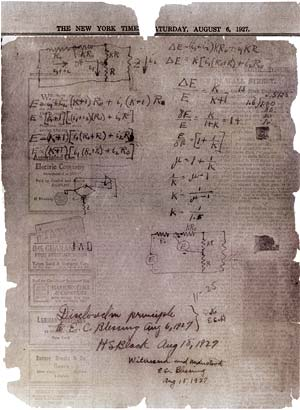
\includegraphics[width=.5\columnwidth]{image_1.jpg} &
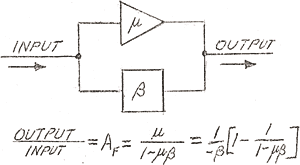
\includegraphics[width=.4\columnwidth]{image_2.png}\\
(a) & (b)\\
\end{tabular}
\caption{Harold Black's original ``back of the envelope" calculations that led to the invention of electronic feedback amplifiers.}
\label{fig:image_1.jpg}
\end{figure}
%%%%%%%%%%%%%%%%%%%%%%%%%%%%%%%%%%%%%%%%%%%%%%%%%%%%%%%%%%%%%%%%%%%%%%%%%%%%%%%%%%%%%%%%
%%%%%%%%%%%%%%%%%%%%%%%%%%%%%%%%%%%%%%%%%%%%%%%%%%%%%%%%%%%%%%%%%%%%%%%%%%%%%%%%%%%%%%%%
%                                   SECTION 17.3                                       %
%%%%%%%%%%%%%%%%%%%%%%%%%%%%%%%%%%%%%%%%%%%%%%%%%%%%%%%%%%%%%%%%%%%%%%%%%%%%%%%%%%%%%%%%
%%%%%%%%%%%%%%%%%%%%%%%%%%%%%%%%%%%%%%%%%%%%%%%%%%%%%%%%%%%%%%%%%%%%%%%%%%%%%%%%%%%%%%%%
\section{Why Feedback?}
%%%%%%%%%%%%%%%%%%%%%%%%%%%%%%%%%%%%%%%%%%%%
%             SUBSECTION 17.3.1            %
%%%%%%%%%%%%%%%%%%%%%%%%%%%%%%%%%%%%%%%%%%%%
\subsection{Precision Analog}
As already noted, feedback allows us to use a really ``crappy" open-loop amplifier and still get good performance in a closed-loop feedback system, as long as the crappy amplifier has high gain.  When the gain is sufficiently high, the gain is determined by the feedback network, not the open-loop gain.  So the open loop gain can vary over temperature, process, it can age, and it can be highly non-linear.  In the end, if the gain is high enough, it does not play a role!
%%%%%%%%%%%%%%%%%%%%%%%%%%%%%%%%%%%%%%%%%%%%
%             SUBSECTION 17.3.2            %
%%%%%%%%%%%%%%%%%%%%%%%%%%%%%%%%%%%%%%%%%%%%
\subsection{Other Benefits of Feedback}
In a feedback system, the closed-loop gain depends on the passive feedback network, which is set precisely using well defined components such as resistors.  It's also dependent on a ratio of resistors, which helps to reduce effects of temperature variations or aging.  It's also important to realize that the op-amp does not even need to be particularly linear.  In fact, when an amplifier has a very high gain, say a million, and is running on a supply voltage of say 5V, then any signal larger than 5$\mu$V will saturate the amplifier, as illustrated in \emph{Fig.~\ref{fig:opamp_fb_precise}}b.  How is it possible to make such a non-linear amplifier behave linearly?  Well, recall that the op-amp processes the error signal, not the input signal, and the corresponding error signal will be very small, and restricted to the linear range of the op-amp, which results in a closed-loop system with very precise gain over a large range of inputs.  So overall the op-amp transfer function is almost perfectly linear, despite using a very non-linear core amplifier. 
%%%%%%%%%%%%%%%%%%%%%%%%%%%%%%%%%%%%%%%%%%%%
In the next section, we'll highlight other important benefits, such as bandwidth enhancement.  
%%%%%%%%%%%%%%%%%%%%%%%%%%%%%%%%%%%%%%%%%%%%
%                 FIGURE                   %
%%%%%%%%%%%%%%%%%%%%%%%%%%%%%%%%%%%%%%%%%%%%
\begin{figure}[tb]
\centering
\begin{tabular}{cc}
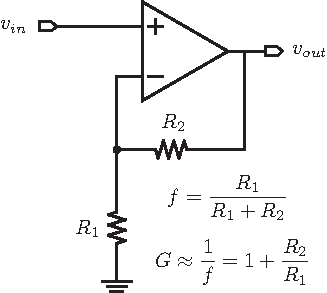
\includegraphics[width=.2\columnwidth]{opamp_fb_precise} &
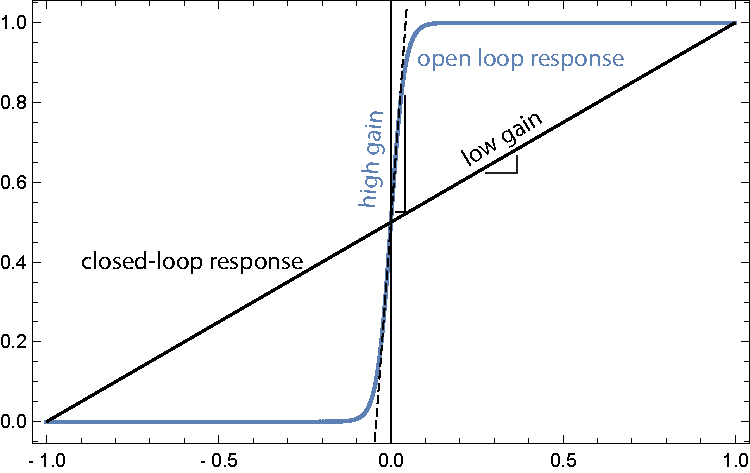
\includegraphics[width=.7\columnwidth]{opamp_gain}\\
(a) & (b) 
\end{tabular}
\caption{(a)  A precision gain stage is realized with a feedback amplifier using an amplifier described by a very non-linear input-output transfer curve, shown in (b).  The system is linear because it transforms a high gain non-linear amplifier into a lower gain linear system by exercising the amplifier with small inputs (error signal).}
\label{fig:opamp_fb_precise}
\end{figure}
%%%%%%%%%%%%%%%%%%%%%%%%%%%%%%%%%%%%%%%%%%%%
%             SUBSECTION 17.3.3            %
%%%%%%%%%%%%%%%%%%%%%%%%%%%%%%%%%%%%%%%%%%%%
\subsection{Loop Gain}
%%%%%%%%%%%%%%%%%%%%%%%%%%%%%%%%%%%%%%%%%%%%
%                 FIGURE                   %
%%%%%%%%%%%%%%%%%%%%%%%%%%%%%%%%%%%%%%%%%%%%
\begin{figure}[tb]
\centering
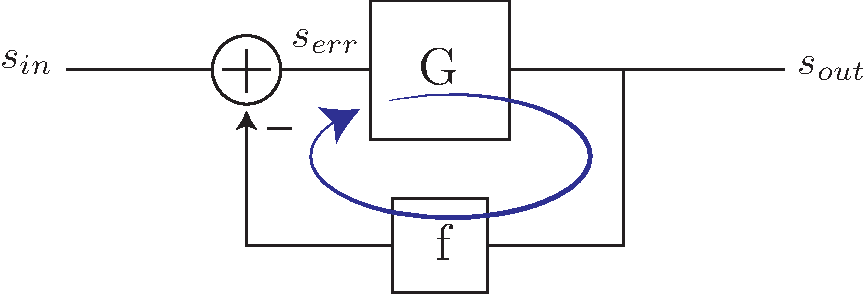
\includegraphics[scale=.7]{fbblock_loopgain}
\caption{The loop gain $T$ is defined as the gain around the loop as shown.}
\label{fig:fbblock_loopgain}
\end{figure}
%%%%%%%%%%%%%%%%%%%%%%%%%%%%%%%%%%%%%%%%%%%%
We have seen that many of the benefits of feedback occur when the gain is large.  More precisely, if we examine the closed-loop transfer function:
    \begin{equation}
        {G_{closed}} = \frac{G}{{1 + Gf}} = \frac{G}{{1 + T}}
    \end{equation}
where $T = Gf$, we see that it's important for $T$ to be large, not just $G$.  $T$ is called the \textbf{loop gain}\index{Loop gain}, because it is the gain going around the loop, shown in \emph{Fig.~\ref{fig:fbblock_loopgain}}.  For a precise transfer function, the key to feedback is to realize sufficiently high loop gain:
    \begin{equation}
        T = Gf \gg 1
    \end{equation}
\newpage
%%%%%%%%%%%%%%%%%%%%%%%%%%%%%%%%%%%%%%%%%%%%
%             SUBSECTION 17.3.4            %
%%%%%%%%%%%%%%%%%%%%%%%%%%%%%%%%%%%%%%%%%%%%
\subsection{Noise Rejection}
%%%%%%%%%%%%%%%%%%%%%%%%%%%%%%%%%%%%%%%%%%%%
%                 FIGURE                   %
%%%%%%%%%%%%%%%%%%%%%%%%%%%%%%%%%%%%%%%%%%%%
\begin{figure}[tb]
\centering
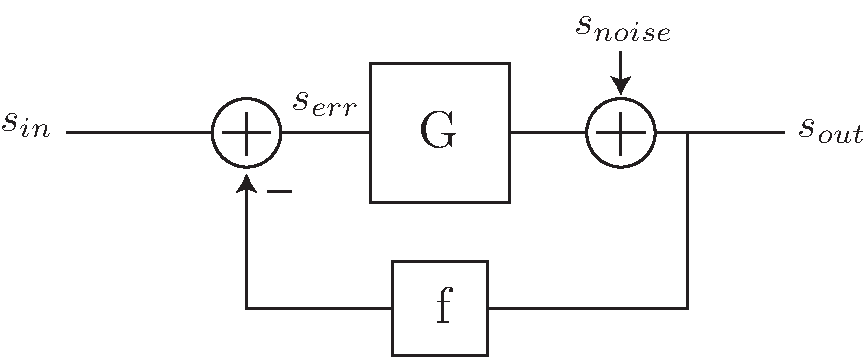
\includegraphics[scale=.7]{fbblock_noise}
\caption{Any noise or distortion injected at the output of the amplifier is rejected by the loop gain of the amplifier.}
\label{fig:fbblock_noise}
\end{figure}
%%%%%%%%%%%%%%%%%%%%%%%%%%%%%%%%%%%%%%%%%%%%
Now consider the effect of injecting interference or noise into a feedback system, as shown in \emph{Fig.~\ref{fig:fbblock_noise}}. \textbf{Interference rejection}\index{Interference!rejection} means that the loop can correct for unwanted signals that are injected into the signal path.  Imagine an unwanted signal couples into the loop as shown.  The transfer function can be derived again:
    \begin{equation}
        {s_{out}} = G{s_{err}} + {s_{noise}} = G({s_{in}} - f{s_{out}}) + {s_{noise}}
    \end{equation}
Collecting $s_{out}$ terms:
    \begin{equation}
        {s_{out}} = \frac{G}{{1 + T}}{s_{in}} + \frac{1}{{1 + T}}{s_{noise}}
    \end{equation}
If $T \gg 1$, then the noise is rejected by $1/(1+T)$. Any unwanted signal, including distortion, is rejected by the loop.
%%%%%%%%%%%%%%%%%%%%%%%%%%%%%%%%%%%%%%%%%%%%
%             SUBSECTION 17.3.5            %
%%%%%%%%%%%%%%%%%%%%%%%%%%%%%%%%%%%%%%%%%%%%
\subsection{Positive Feedback}
%%%%%%%%%%%%%%%%%%%%%%%%%%%%%%%%%%%%%%%%%%%%
%                 FIGURE                   %
%%%%%%%%%%%%%%%%%%%%%%%%%%%%%%%%%%%%%%%%%%%%
\begin{figure}[tb]
\centering
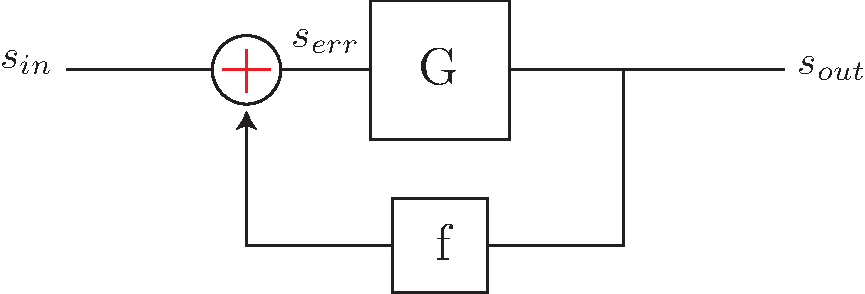
\includegraphics[scale=.7]{fbblock_posfb}
\caption{The block diagram of a positive feedback system.}
\label{fig:fbblock_posfb}
\end{figure}
%%%%%%%%%%%%%%%%%%%%%%%%%%%%%%%%%%%%%%%%%%%%
Up to now we have been considering a \textbf{negative feedback}\index{Feedback!negative} system, whereby the output is subtracted from the input. If we were to add the output to the input, the system would be a \textbf{positive feedback}\index{Feedback!positive} system, as shown in \emph{Fig.~\ref{fig:fbblock_posfb}}.

Positive feedback is also useful and has applications, but they are very different.  For example, positive feedback systems tend to “rail out”, in other words they can be regenerative.  This is great for building \textbf{hysteresis}\index{Hysteresis} or a memory element, and indeed a basic SRAM cell is a positive feedback loop involving two CMOS inverters.  Positive feedback systems can still be designed to provide gain, but the loop gain should be less than unity, $T < 1$.  The reason for this are clear if we imagine that the current output is the input gained up, plus an infinite number of copies that go around the loop and add to the output.  This is exactly a \textbf{geometric series}\index{Series!geometric}\footnote{See appendix ~\ref{sec:geometric} for a review of the geometric series.}, and it converges as long as $T< 1$, and it converges to a value of
    \begin{equation}
        G_{closed} = G \cdot \sum_{i=0}^\infty T^i = \frac{G}{1 - T}
    \end{equation}
The benefit over negative feedback is that positive feedback can boost the gain, and in fact if we make $T = 1 - \epsilon$, where $\epsilon$ is a small number, we can make an arbitrarily large gain.  The danger is that the gain is hard to control and can easily result in $T > 1$, causing a completely different behavior (such as oscillation or railing out).  In practice, in the design of linear analog circuits, positive feedback is used sparingly.  When positive feedback is used, the designer must be aware of the feedback loop and ensure that under all conditions the loop gain does not exceed $1$.
%%%%%%%%%%%%%%%%%%%%%%%%%%%%%%%%%%%%%%%%%%%%%%%%%%%%%%%%%%%%%%%%%%%%%%%%%%%%%%%%%%%%%%%%
%%%%%%%%%%%%%%%%%%%%%%%%%%%%%%%%%%%%%%%%%%%%%%%%%%%%%%%%%%%%%%%%%%%%%%%%%%%%%%%%%%%%%%%%
%                                   SECTION 17.4                                       %
%%%%%%%%%%%%%%%%%%%%%%%%%%%%%%%%%%%%%%%%%%%%%%%%%%%%%%%%%%%%%%%%%%%%%%%%%%%%%%%%%%%%%%%%
%%%%%%%%%%%%%%%%%%%%%%%%%%%%%%%%%%%%%%%%%%%%%%%%%%%%%%%%%%%%%%%%%%%%%%%%%%%%%%%%%%%%%%%%
\section{Circuit Models for Op-Amps}
%%%%%%%%%%%%%%%%%%%%%%%%%%%%%%%%%%%%%%%%%%%%
%             SUBSECTION 17.4.1            %
%%%%%%%%%%%%%%%%%%%%%%%%%%%%%%%%%%%%%%%%%%%%
\subsection{Practical Op-Amps}
Let's now delve into the details of building feedback systems based on op-amps.  We need a way to model real op-amps, and we can categorize the op-amp's imperfections into two categories.  First, let's consider ``linear" imperfections. In other words, things that we can include into a linear model.  These include:
    \begin{itemize}
        \item  Finite open-loop gain ($A_0 < \infty$)
        \item  Finite input resistance ($R_i < \infty\Omega$)
     	\item Non-zero output resistance ($R_0 > 0\Omega$ )
     	\item Finite bandwidth and the gain-bandwidth trade-off (to be discussed) 
    \end{itemize}
There are other non-linear imperfections that we'll discuss in the next chapter.  These include:
    \begin{itemize}
        \item Slew rate limitations (explained in the next chapter)
        \item Finite swing
        \item Offset voltage
        \item Input bias and offset currents
        \item Noise and distortion
    \end{itemize}
Even though noise can be treated as a linear phenomena, for convenience we'll discuss it in the next chapter.  So our goal is to build a model that contains as many of these imperfections as possible, while keeping the model simple and easy to use as possible.
%%%%%%%%%%%%%%%%%%%%%%%%%%%%%%%%%%%%%%%%%%%%
%             SUBSECTION 17.4.2            %
%%%%%%%%%%%%%%%%%%%%%%%%%%%%%%%%%%%%%%%%%%%%
\subsection{World's Simplest Op-Amp Model}
%%%%%%%%%%%%%%%%%%%%%%%%%%%%%%%%%%%%%%%%%%%%
%                 FIGURE                   %
%%%%%%%%%%%%%%%%%%%%%%%%%%%%%%%%%%%%%%%%%%%%
\begin{figure}[tb]
\centering
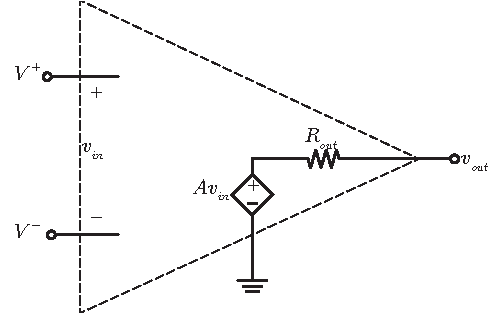
\includegraphics[scale=1]{opamp_model}
\caption{A simple model for an op-amp.}
\label{fig:opamp_model}
\end{figure}
%%%%%%%%%%%%%%%%%%%%%%%%%%%%%%%%%%%%%%%%%%%%
The world's simplest op-amp model is shown in \emph{Fig.~\ref{fig:opamp_model}}. This is the ``VCVS'' model, or the \textbf{Voltage-Controlled Voltage Source}\index{Voltage source!Voltage-controlled} model.  While it captures finite gain and output resistance, it fails to capture frequency dependence.
%%%%%%%%%%%%%%%%%%%%%%%%%%%%%%%%%%%%%%%%%%%%
%             SUBSECTION 17.4.3            %
%%%%%%%%%%%%%%%%%%%%%%%%%%%%%%%%%%%%%%%%%%%%
\subsection{General Model of Amplifier}
%%%%%%%%%%%%%%%%%%%%%%%%%%%%%%%%%%%%%%%%%%%%
%                 FIGURE                   %
%%%%%%%%%%%%%%%%%%%%%%%%%%%%%%%%%%%%%%%%%%%%
\begin{figure}[tb]
\centering
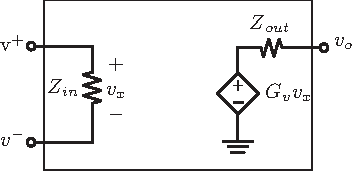
\includegraphics[scale=1]{vampmodelz}
\caption{A general model for any voltage amplifier, including an op-amp, includes frequency dependent elements that make the model unsuitable for analysis.}
\label{fig:vampmodelz}
\end{figure}
%%%%%%%%%%%%%%%%%%%%%%%%%%%%%%%%%%%%%%%%%%%%
While it's easy to build a model that can take into account input impedance $Z_{in}(j\omega)$, output impedance $Z_{out}(j\omega)$, and frequency dependent finite gain $G_v(j\omega)$, using such a general model shown in \emph{Fig.~\ref{fig:vampmodelz}} is too complicated, as all the parameters vary with frequency.  This model also fails to provide any insights and is too general for our purposes.  Let's build a ``single-pole" (dominant pole) model by taking the frequency dependence away from $G_v$.
%%%%%%%%%%%%%%%%%%%%%%%%%%%%%%%%%%%%%%%%%%%%
%             SUBSECTION 17.4.4            %
%%%%%%%%%%%%%%%%%%%%%%%%%%%%%%%%%%%%%%%%%%%%
\subsection{``Physical" Op-Amp Model}
%%%%%%%%%%%%%%%%%%%%%%%%%%%%%%%%%%%%%%%%%%%%
%                 FIGURE                   %
%%%%%%%%%%%%%%%%%%%%%%%%%%%%%%%%%%%%%%%%%%%%
\begin{figure}[tb]
\centering
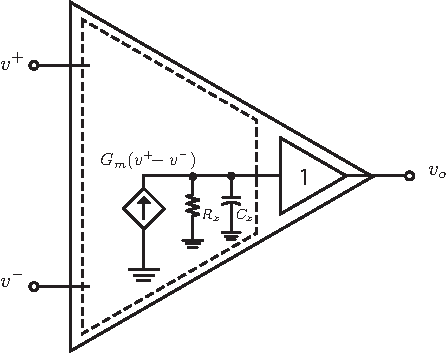
\includegraphics[scale=1]{opamp_model_pole}
\caption{An op-amp model with a single pole is inspired from the physical structure of an actual transistor based op-amp.}
\label{fig:opamp_model_pole}
\end{figure}
%%%%%%%%%%%%%%%%%%%%%%%%%%%%%%%%%%%%%%%%%%%%
The model shown in \emph{Fig.~\ref{fig:opamp_model_pole}}, uses a $G_m$ cell, or an \textbf{ideal transconductor}\index{Transconductor!ideal}.  We learned that a differential pair can be modeled as a $G_m$ cell, and so as you might expect, the input stage of almost every op-amp is a differential pair.  The DC gain and dominant op-amp pole is modeled by $R_x$ and $C_x$.  The larger $R_x$, the larger the DC gain $A_0 = G_m R_x$.  The output resistance can be added easily at the output of the ideal voltage buffer (unity gain amp).
\newpage
%%%%%%%%%%%%%%%%%%%%%%%%%%%%%%%%%%%%%%%%%%%%
%             SUBSECTION 17.4.5            %
%%%%%%%%%%%%%%%%%%%%%%%%%%%%%%%%%%%%%%%%%%%%
\subsection{Operational Transconductance Amplifier (OTA)}
%%%%%%%%%%%%%%%%%%%%%%%%%%%%%%%%%%%%%%%%%%%%
%                 FIGURE                   %
%%%%%%%%%%%%%%%%%%%%%%%%%%%%%%%%%%%%%%%%%%%%
\begin{figure}[tb]
\centering
\begin{tabular}{cc}
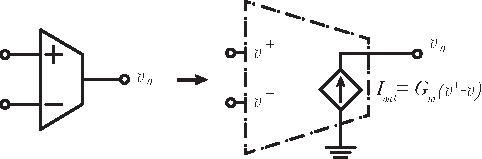
\includegraphics[scale=1]{OTA} &
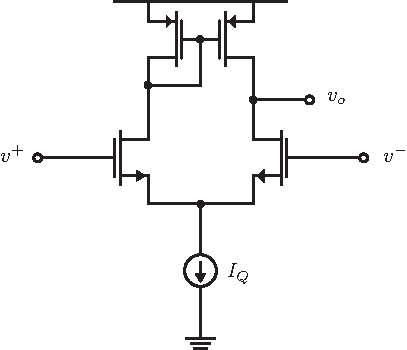
\includegraphics[width=.3\columnwidth]{Diffpair_se_output.pdf}\\
(a) & (b)\\
\end{tabular}
\caption{(a) An Operational Transconductance Amplifier (OTA) forms the input stage of an op-amp.  (b) It is realized using a differential pair with mirror load, or a similar circuit.}
\label{fig:OTA}
\end{figure}
%%%%%%%%%%%%%%%%%%%%%%%%%%%%%%%%%%%%%%%%%%%%
Notice that if you ``slice off" the triangular head of an op-amp, the result is the transconductance stage (see dashed lines in \emph{Fig.~\ref{fig:opamp_model_pole}}), and has a special symbol shown in \emph{Fig.~\ref{fig:OTA}}a.  It is known as an \textbf{Operational Transconductance Amplifier}\index{Amplifier!Operational transconductance}, also known as an ``OTA".  An OTA is essentially a differential transistor pair with a high output impedance node, for example using a mirror as shown in \emph{Fig.~\ref{fig:OTA}}b.
%%%%%%%%%%%%%%%%%%%%%%%%%%%%%%%%%%%%%%%%%%%%
Since an OTA is essentially a $G_m$ amplifier, it converts a differential voltage into an output current.  So if we want to drive a load resistor, we need an output stage (buffer).  As such, many real op-amps are internally constructed from an OTA + buffer as shown.
%%%%%%%%%%%%%%%%%%%%%%%%%%%%%%%%%%%%%%%%%%%%
%             SUBSECTION 17.4.6            %
%%%%%%%%%%%%%%%%%%%%%%%%%%%%%%%%%%%%%%%%%%%%
\subsection{Op-Amp Capacitance}
%%%%%%%%%%%%%%%%%%%%%%%%%%%%%%%%%%%%%%%%%%%%
%                 FIGURE                   %
%%%%%%%%%%%%%%%%%%%%%%%%%%%%%%%%%%%%%%%%%%%%
\begin{figure}[tb]
\centering
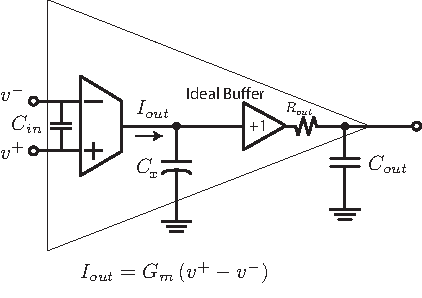
\includegraphics[scale=1]{opamp_ota_model_cap}
\caption{Op-amp model with infinite gain and output impedance.  The role of the capacitance $C_x$ is to model the frequency response of the amplifier.}
\label{fig:opamp_ota_model_cap}
\end{figure}
%%%%%%%%%%%%%%%%%%%%%%%%%%%%%%%%%%%%%%%%%%%%
In \emph{Fig.~\ref{fig:opamp_ota_model_cap}}, we've added input capacitance and output capacitance to the basic model.  Since $R_x$ is absent, the DC gain is infinite.  This is also known as an \textbf{integrator}\index{Op-amp!integrator}, because the voltage at the output is an integral of the differential voltage.    
%%%%%%%%%%%%%%%%%%%%%%%%%%%%%%%%%%%%%%%%%%%%
What is the origin of $C_{in}$ and $C_{out}$?  Any amplifier has input/output capacitance due to transistors and packaging parasitics.  The capacitance also arises from cables or long board traces.  In some cases the sensor or actuator of interest (the source or load) has a capacitive component. Note that without $R_{out}$, the output capacitance has no impact on the transfer function.  In other words, an ideal buffer can drive any load.  For the focus of the rest of the chapter, we'll zoom in on the internal capacitance $C_x$.
\newpage
%%%%%%%%%%%%%%%%%%%%%%%%%%%%%%%%%%%%%%%%%%%%
%             SUBSECTION 17.4.7            %
%%%%%%%%%%%%%%%%%%%%%%%%%%%%%%%%%%%%%%%%%%%%
\subsection{Transconductance Amplifier Model}
%%%%%%%%%%%%%%%%%%%%%%%%%%%%%%%%%%%%%%%%%%%%
%                 FIGURE                   %
%%%%%%%%%%%%%%%%%%%%%%%%%%%%%%%%%%%%%%%%%%%%
\begin{figure}[tb]
\centering
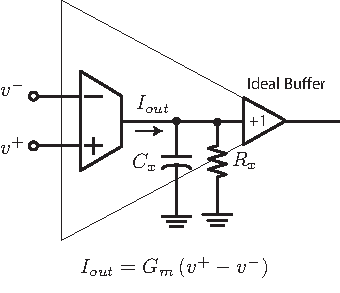
\includegraphics[width=.5\columnwidth]{opamp_ota_model_gain}
\caption{Op-amp model with finite DC gain and a single pole. This model is equivalent to \emph{Fig.~\ref{fig:opamp_model_pole}}.}
\label{fig:opamp_ota_model_gain}
\end{figure}

The OTA model shown in \emph{Fig.~\ref{fig:opamp_ota_model_gain}} closely resembles the insides of an op-amp.  The only difference between this model and \emph{Fig.~\ref{fig:opamp_model_pole}} is notation.  We've used the OTA symbol for the input $G_m$.  To get high gain, the input $G_m$ drives a high impedance $Z$ node (formed by $C_x$ and $R_x$). The output buffer is provided to drive a low impedance load and to preserve the high voltage gain.  This model includes the first pole of the amplifier.
%\subsection{Redrawn Op-Amp Model (Infinite Gain)}
%
%\begin{figure}[tb]
%\centering
%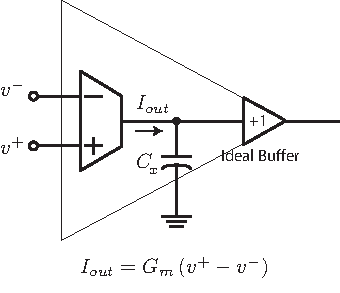
\includegraphics[scale=1]{opamp_ota_model}
%\caption{opamp ota model} \label{fig:opamp_ota_model}
%\end{figure}
%
% In this ideal model, we set $R_x$ to infinity and have infinite DC gain.  
% Again, the differential $G_m$ cell is represented by a funny looking amplifier symbol.  Where does this symbol come from?
%%%%%%%%%%%%%%%%%%%%%%%%%%%%%%%%%%%%%%%%%%%%%%%%%%%%%%%%%%%%%%%%%%%%%%%%%%%%%%%%%%%%%%%%
%%%%%%%%%%%%%%%%%%%%%%%%%%%%%%%%%%%%%%%%%%%%%%%%%%%%%%%%%%%%%%%%%%%%%%%%%%%%%%%%%%%%%%%%
%                                   SECTION 17.5                                       %
%%%%%%%%%%%%%%%%%%%%%%%%%%%%%%%%%%%%%%%%%%%%%%%%%%%%%%%%%%%%%%%%%%%%%%%%%%%%%%%%%%%%%%%%
%%%%%%%%%%%%%%%%%%%%%%%%%%%%%%%%%%%%%%%%%%%%%%%%%%%%%%%%%%%%%%%%%%%%%%%%%%%%%%%%%%%%%%%%
\section{Gain/Bandwidth Trade-off}
%%%%%%%%%%%%%%%%%%%%%%%%%%%%%%%%%%%%%%%%%%%%
%             SUBSECTION 17.5.1            %
%%%%%%%%%%%%%%%%%%%%%%%%%%%%%%%%%%%%%%%%%%%%
\subsection{Op-Amp Gain / Bandwidth}
%%%%%%%%%%%%%%%%%%%%%%%%%%%%%%%%%%%%%%%%%%%%
%                 FIGURE                   %
%%%%%%%%%%%%%%%%%%%%%%%%%%%%%%%%%%%%%%%%%%%%
\begin{figure}[tb]
\centering
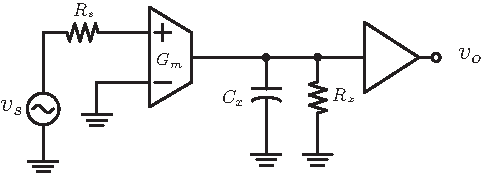
\includegraphics[scale=1]{ota_amp_open}
\caption{The open loop gain and bandwidth of the op-amp model is calculated using the OTA op-amp model by driving the positive input with a source and observing the output voltage.}
\label{fig:ota_amp_open}
\end{figure}
%%%%%%%%%%%%%%%%%%%%%%%%%%%%%%%%%%%%%%%%%%%%
Consider the \textbf{open-loop amplifier}\index{Amplifier!open-loop} shown in \emph{Fig.~\ref{fig:ota_amp_open}}.  Using the concept of impedance, it's easy to derive the transfer function and verify that it is a first-order single pole system.

\vspace{0.15cm}
\noindent
At DC the capacitor becomes an open circuit, and the gain is simply:
    \begin{equation}
        G_0 = {G_m}{R_x}
    \end{equation}
The dominant frequency response of the op-amp is due to the time constant formed at the high-$Z$ node:
    \begin{equation}
        \omega _{ - 3dB} = 1/{R_x}{C_x}
    \end{equation}
An interesting observation is that the \textbf{gain-bandwidth product}\index{Gain-bandwidth product} depends on only on $G_m$ and $C_x$ (and not the gain $G_0$): 
    \begin{equation}
        G_0 \times {\omega _{ - 3dB}} = \frac{{{G_m}}}{{{C_x}}}
    \end{equation}
%%%%%%%%%%%%%%%%%%%%%%%%%%%%%%%%%%%%%%%%%%%%
%             SUBSECTION 17.5.2            %
%%%%%%%%%%%%%%%%%%%%%%%%%%%%%%%%%%%%%%%%%%%%
\subsection{Driving Capacitive Loads}
%%%%%%%%%%%%%%%%%%%%%%%%%%%%%%%%%%%%%%%%%%%%
%                 FIGURE                   %
%%%%%%%%%%%%%%%%%%%%%%%%%%%%%%%%%%%%%%%%%%%%
\begin{figure}[tb]
\centering
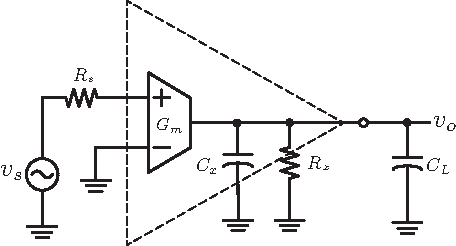
\includegraphics[scale=1]{ota_amp_capload}
\caption{When an op-amp drives a capacitive load, the internal buffer can be eliminated.  In this case, the bandwidth is determined by a combination of the internal capacitance and the load capacitance $C_L$.}
\label{fig:ota_amp_capload}
\end{figure}
%%%%%%%%%%%%%%%%%%%%%%%%%%%%%%%%%%%%%%%%%%%%
In many situations, the load is a capacitor rather than a resistor, as shown in \emph{Fig.~\ref{fig:ota_amp_capload}}.
%%%%%%%%%%%%%%%%%%%%%%%%%%%%%%%%%%%%%%%%%%%%
For such cases, we can directly use an OTA (rather than a full op-amp) and the bandwidth is determined by the load capacitance
    \begin{equation}
        {\omega _{ - 3dB}} = \frac{1}{{{R_x}({C_x} + {C_L})}}
    \end{equation}
%\begin{equation}
%	G = {G_m}{R_x}
%\end{equation}
%
%\subsection{OTA Power Consumption}
%
% For a fixed load, the current consumption of the OTA is usually determined by the gain/bandwidth requirement, assuming load dominates
%\begin{equation}
%	C_L \gg C_x
%\end{equation}
% $G_m$ scales with current, so driving a larger capacitance requires more power
%%%%%%%%%%%%%%%%%%%%%%%%%%%%%%%%%%%%%%%%%%%%
%             SUBSECTION 17.5.3            %
%%%%%%%%%%%%%%%%%%%%%%%%%%%%%%%%%%%%%%%%%%%%
\subsection{Open-Loop Frequency Response}
%%%%%%%%%%%%%%%%%%%%%%%%%%%%%%%%%%%%%%%%%%%%
%                 FIGURE                   %
%%%%%%%%%%%%%%%%%%%%%%%%%%%%%%%%%%%%%%%%%%%%
\begin{figure}[tb]
\centering
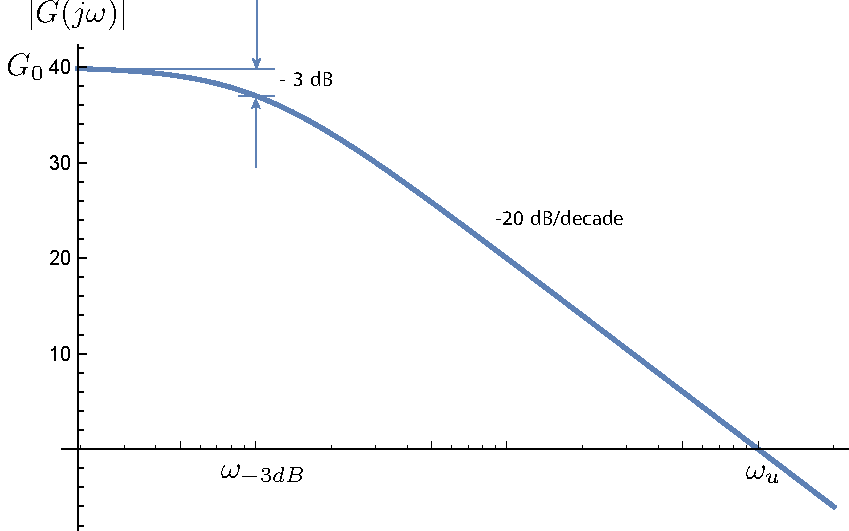
\includegraphics[width=.7\columnwidth]{mag1pole}
\caption{The magnitude response of a single pole op-amp.  Note the gain is unity at the frequency $\omega_u$.}
\label{fig:mag1pole}
\end{figure}
%%%%%%%%%%%%%%%%%%%%%%%%%%%%%%%%%%%%%%%%%%%%
A plot of the single-pole frequency response is shown in \emph{Fig.~\ref{fig:mag1pole}}.  The DC gain $G_0$ and the 3-dB frequency $\omega_{\text{-3dB}}$ completely define the transfer function.  We will also highlight another important quantity known as the \textbf{unity gain frequency}\index{Unity-gain frequency}, $\omega_u$.  This is the frequency at which the transfer function has unit magnitude:
    \begin{equation}
        |G(j\omega_u )| = \left| \frac{G_0}{1 + j\omega_u/\omega_{\text{-3dB}}} \right| = 1
    \end{equation}
To find it, note that the transfer function beyond $\omega_{\text{-3dB}}$, or for $\omega \gg \omega_{\text{-3dB}}$, the closed-loop gain can be simplified:
    \begin{equation}
        |G(j\omega_u )| \approx G_0 \left| \frac{1}{j\omega_u/\omega_{\text{-3dB}}} \right| = G_0 \frac{\omega_{\text{-3dB}}}{\omega_u} = 1 
    \end{equation}
In other words, the unity gain frequency is given by:
    \begin{equation}
        \omega_u \approx G_0 \omega_{\text{-3dB}}
    \end{equation}  
This also shows that the gain at high frequencies is given by:
    \begin{equation}
        G(j\omega ) \approx \frac{{{\omega_u}}}{{j\omega }}
    \end{equation}
The unity gain frequency or bandwidth is also known as the gain-bandwidth product for obvious reasons.   The unity gain frequency plays a prominent role in the frequency response of amplifiers.
%%%%%%%%%%%%%%%%%%%%%%%%%%%%%%%%%%%%%%%%%%%%
%             SUBSECTION 17.5.4            %
%%%%%%%%%%%%%%%%%%%%%%%%%%%%%%%%%%%%%%%%%%%%
\subsection{Bandwidth Extension}
To see why the unity gain is important, consider again a core amplifier with a single pole.  The transfer function is given by:
    \begin{equation}
        G(j\omega ) = \frac{{{G_0}}}{{1 + j\omega \tau }}
    \end{equation}
where for convenience we're using $\tau = 1/\omega_{\text{-3dB}}$, also known as the time constant of the system.  We know that the step response of the amplifier is dominated by $\tau$, which is inverse of the bandwidth.  When we use this amplifier in feedback, the overall transfer function is given by:
    \begin{equation}
        G_{CL} (j\omega ) = \frac{G(j\omega )}{1 +G(j\omega )f } = \frac{\frac{{{G_0}}}{{1 + j\omega \tau }}}{1 + \frac{{{G_0 f}}}{{1 + j\omega \tau }} }
    \end{equation}
If we clear the common fraction $(1 + j\omega \tau)$:
    \begin{equation}
        G_{CL} (j\omega ) = \frac{G_0}{(1 + j\omega \tau) + G_0 f  }
    \end{equation}
Finally, we put the equation in standard form to read off the bandwidth:
    \begin{equation}
        G_{CL} (j\omega) = \frac{\frac{G_0}{1 + T}}{1 + j\omega \frac{\tau}{1+T}}
    \end{equation}
The amplifier step response is faster by the factor $(1+T)$, or approximately by the loop gain ($T = G_0 f \gg 1$).  We can equivalently say that the bandwidth $\omega_0$ of the closed loop amplifier has expanded by $(1+T)$:
    \begin{equation}
        \omega_0 = \frac{(1+T)}{\tau} = (1 + T) \omega_{\text{-3dB}}
    \end{equation}
\newpage
%%%%%%%%%%%%%%%%%%%%%%%%%%%%%%%%%%%%%%%%%%%%
%             SUBSECTION 17.5.5            %
%%%%%%%%%%%%%%%%%%%%%%%%%%%%%%%%%%%%%%%%%%%%
\subsection{Gain / Bandwidth Product in Feedback}
%%%%%%%%%%%%%%%%%%%%%%%%%%%%%%%%%%%%%%%%%%%%
%                 FIGURE                   %
%%%%%%%%%%%%%%%%%%%%%%%%%%%%%%%%%%%%%%%%%%%%
\begin{figure}[tb]
\centering
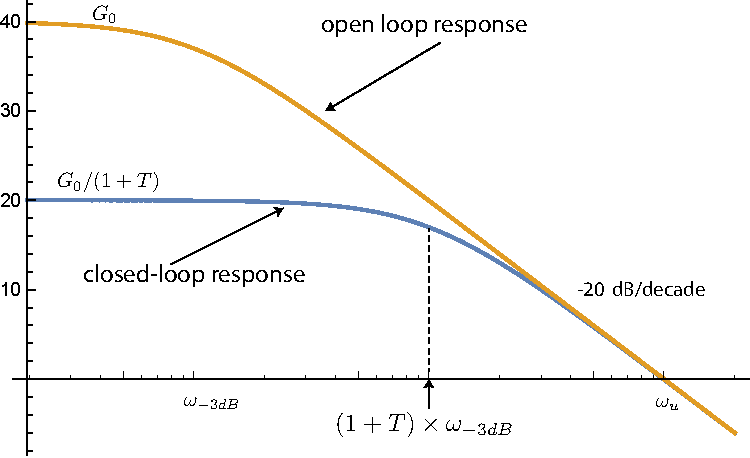
\includegraphics[width=.7\columnwidth]{mag1pole_fb}
\caption{The magnitude response of an op-amp amplifier in closed-loop configuration compared to the original open-loop response.}
\label{fig:mag1pole_fb}
\end{figure}
%%%%%%%%%%%%%%%%%%%%%%%%%%%%%%%%%%%%%%%%%%%%
Both the open-loop and closed-loop transfer function are shown in \emph{Fig.~\ref{fig:mag1pole_fb}}.  Even though the bandwidth expanded by $(1+T)$, the gain drops by the same factor. So overall the gain-bandwidth ($GBW$) product is constant. The $GBW$ product depends only the the $G_m$ of the op-amp and the $C_x$ internal capacitance (or load in the case of an OTA):
    \begin{equation}
        \omega_u = GBW = G_0 \cdot \omega_{\text{-3dB}}  = G_m R_x \cdot \frac{1}{C_x R_x} = \frac{G_m}{C_x}
    \end{equation} 
In other words, even for an on-amp with infinite gain, shown in \emph{Fig.~\ref{fig:opamp_ota_model_gain}}, the gain-bandwidth product is the same.  Since the frequency response of the closed loop system is determined by $\omega_u$, it's common to specify the $GBW$ of an op-amp rather than its open-loop bandwidth.  To determine the closed-loop bandwidth, all we have to take the product of the feedback factor $f$ and $\omega_u$:
    \begin{equation}
        \omega_0 = f T
    \end{equation} 
%%%%%%%%%%%%%%%%%%%%%%%%%%%%%%%%%%%%%%%%%%%%
%             SUBSECTION 17.5.6            %
%%%%%%%%%%%%%%%%%%%%%%%%%%%%%%%%%%%%%%%%%%%%
\subsection{Unity Gain Feedback Amplifier}
%%%%%%%%%%%%%%%%%%%%%%%%%%%%%%%%%%%%%%%%%%%%
%                 FIGURE                   %
%%%%%%%%%%%%%%%%%%%%%%%%%%%%%%%%%%%%%%%%%%%%
\begin{figure}[tb]
\centering
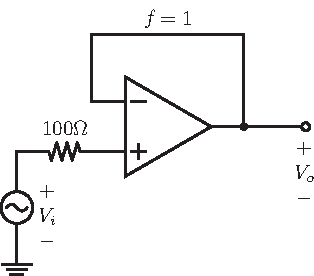
\includegraphics[scale=1]{opamp_unitygain}
\caption{An op-amp configured in unity-gain configuration.  Note the feedback factor is unity rendering the closed-loop bandwidth $\omega_0 = \omega_u = GBW$.}
\label{fig:opamp_unitygain}
\end{figure}
%%%%%%%%%%%%%%%%%%%%%%%%%%%%%%%%%%%%%%%%%%%%
Consider a voltage follower feedback amplifier, shown in \emph{Fig.~\ref{fig:opamp_unitygain}}.  The amplifier has a feedback factor $f = 1$, and so it has the full $GBW$ product frequency range available, making it a very broadband amplifier.
%%%%%%%%%%%%%%%%%%%%%%%%%%%%%%%%%%%%%%%%%%%%
%             SUBSECTION 17.5.7            %
%%%%%%%%%%%%%%%%%%%%%%%%%%%%%%%%%%%%%%%%%%%%
\subsection{How Feedback Broadbands an Amplifier}
So far we have shown mathematically that feedback extends the bandwidth by the loop gain. In this section, we would like to provide some circuit insight into the behavior.
%%%%%%%%%%%%%%%%%%%%%%%%%%%%%%%%%%%%%%%%%%%%
%             SUBSECTION 17.5.8            %
%%%%%%%%%%%%%%%%%%%%%%%%%%%%%%%%%%%%%%%%%%%%
\subsection{Back to Circuit Model}
%%%%%%%%%%%%%%%%%%%%%%%%%%%%%%%%%%%%%%%%%%%%
%                 FIGURE                   %
%%%%%%%%%%%%%%%%%%%%%%%%%%%%%%%%%%%%%%%%%%%%
\begin{figure}[tb]
\centering
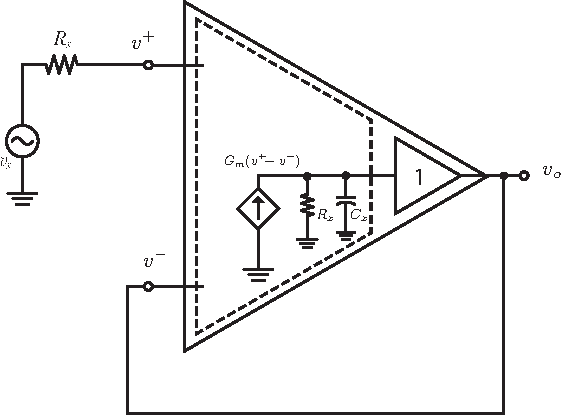
\includegraphics[scale=1]{opamp_model_fb_unity}
\caption{Model of op-amp in unity-gain configuration.}
\label{fig:opamp_model_fb_unity}
\end{figure}
%%%%%%%%%%%%%%%%%%%%%%%%%%%%%%%%%%%%%%%%%%%%
Consider the equivalent circuit for an amplifier with unity gain feedback, shown in \emph{Fig.~\ref{fig:opamp_model_fb_unity}}.  What's the bandwidth?  If you said $1/R_x C_x$, think again!  The dependent current source plays a crucial role.  As far as $C_x$ is concerned, the only resistance is not $R_x$ since we must also consider the dependent source since it's driven by a non-zero control signal.
%%%%%%%%%%%%%%%%%%%%%%%%%%%%%%%%%%%%%%%%%%%%
%             SUBSECTION 17.5.9            %
%%%%%%%%%%%%%%%%%%%%%%%%%%%%%%%%%%%%%%%%%%%%
\subsection{Turning a Current Source into a Resistor}
%%%%%%%%%%%%%%%%%%%%%%%%%%%%%%%%%%%%%%%%%%%%
%                 FIGURE                   %
%%%%%%%%%%%%%%%%%%%%%%%%%%%%%%%%%%%%%%%%%%%%
\begin{figure}[tb]
\centering
\begin{tabular}{cc}
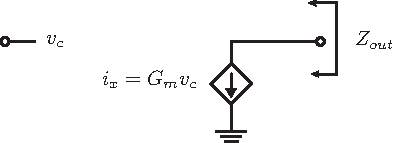
\includegraphics[width=.4\columnwidth]{tia_zout} &
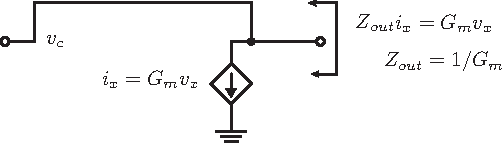
\includegraphics[width=.4\columnwidth]{tia_zout_fb}\\
(a) & (b)\\
\end{tabular}
\caption{(a) The impedance at the output of a transconductor depends on the control voltage. If the control voltage is zero, the output impedance is infinity.  (b) If the control voltage is shorted to the output node, then the transconductor is an ordinary resistor with resistance $1/G_m$.}
\label{fig:tia_zout}
\end{figure}
%%%%%%%%%%%%%%%%%%%%%%%%%%%%%%%%%%%%%%%%%%%%
This problem should be somewhat familiar.  Recall that a MOS diode has an output impedance of $1/g_m$, not $r_o$, because of the drain-gate connection.  As shown in \emph{Fig.~\ref{fig:tia_zout}}, when a \textbf{voltage-controlled current source}\index{Current source!voltage-controlled} has an output impedance that depends on the controlling voltage, it's just a resistor of value $1/G_m$.  Likewise, if we calculate $Z_{out}$ at the internal node of the op-amp, as shown in \emph{Fig.~\ref{fig:opamp_model_fb_unity_label}}, the impedance is much lower than $R_x$.   Here we see the action of the feedback is to lower the impedance seen by the $C_x$ by the loop gain, which expands the bandwidth by the same factor.
    \begin{equation}
        Z_{out} = R_x || \frac{1}{G_m} \approx \frac{1}{G_m}
    \end{equation}
The gain to this node is given by:
    \begin{equation}
        G \approx G_m \cdot \frac{1}{G_m} = 1
    \end{equation}
which makes sense due to the unity gain feedback.  The bandwidth is thus:
    \begin{equation}
        \omega_0 \approx \frac{G_m}{C_x } = \omega_u
    \end{equation}
which matches our derivation earlier.

Now we can see that the action of the feedback is to lower the impedance of the high-$Z$ node, which lowers the gain and expands the bandwidth. It is not hard to show that if the feedback factor is $f$, then the input impedance at the node is approximately given by:
    \begin{equation}
        Z_{out} = R_x || \frac{1}{f G_m} \approx \frac{1}{f G_m}
    \end{equation}
Resulting in a closed-loop gain of 
    \begin{equation}
        G \approx G_m \cdot \frac{1}{f G_m} = \frac{1}{f}
    \end{equation}
and bandwidth:
    \begin{equation}
        \omega_0 \approx \frac{f G_m}{C_x } = f \omega_u  = f G_0 \omega_{\text{-3dB}} = f \omega_u  
    \end{equation}
%%%%%%%%%%%%%%%%%%%%%%%%%%%%%%%%%%%%%%%%%%%%
%                 FIGURE                   %
%%%%%%%%%%%%%%%%%%%%%%%%%%%%%%%%%%%%%%%%%%%%
\begin{figure}[tb]
\centering
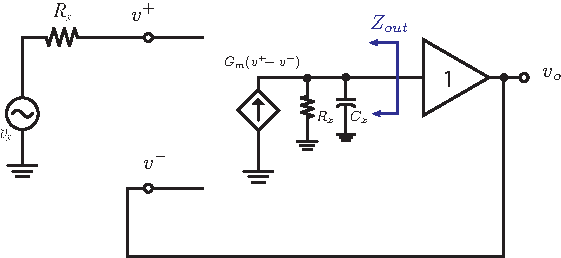
\includegraphics[scale=1]{opamp_model_fb_unity_label}
\caption{The unity-gain feedback in an op-amp causes the high-$Z$ node impedance to drop to $1/G_m$, reducing the gain to unity and expanding the bandwidth.}
\label{fig:opamp_model_fb_unity_label}
\end{figure}
\newpage
%%%%%%%%%%%%%%%%%%%%%%%%%%%%%%%%%%%%%%%%%%%%%%%%%%%%%%%%%%%%%%%%%%%%%%%%%%%%%%%%%%%%%%%%
%%%%%%%%%%%%%%%%%%%%%%%%%%%%%%%%%%%%%%%%%%%%%%%%%%%%%%%%%%%%%%%%%%%%%%%%%%%%%%%%%%%%%%%%
%                                   SECTION 17.6                                       %
%%%%%%%%%%%%%%%%%%%%%%%%%%%%%%%%%%%%%%%%%%%%%%%%%%%%%%%%%%%%%%%%%%%%%%%%%%%%%%%%%%%%%%%%
%%%%%%%%%%%%%%%%%%%%%%%%%%%%%%%%%%%%%%%%%%%%%%%%%%%%%%%%%%%%%%%%%%%%%%%%%%%%%%%%%%%%%%%%
\section{Feedback and Stability}
\label{sec:opamp_stability}
In this section we will only touch upon the important topic of feedback and \textbf{stability}\index{Stability}. In a more advanced course you will analyze feedback and techniques to stabilize an amplifier in detail.
%%%%%%%%%%%%%%%%%%%%%%%%%%%%%%%%%%%%%%%%%%%%
%             SUBSECTION 17.6.1            %
%%%%%%%%%%%%%%%%%%%%%%%%%%%%%%%%%%%%%%%%%%%%
\subsection{Stability}
%%%%%%%%%%%%%%%%%%%%%%%%%%%%%%%%%%%%%%%%%%%%
%                 FIGURE                   %
%%%%%%%%%%%%%%%%%%%%%%%%%%%%%%%%%%%%%%%%%%%%
\begin{figure}[tb]
\centering
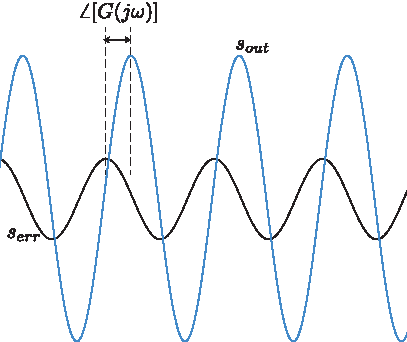
\includegraphics[width=.85\columnwidth]{signal_phase_shift}
\caption{When driven by a sinusoidal voltage, the output voltage is phase delayed with respect to the input by an amount of $\angle G(j\omega)$.}
\label{fig:signal_phase_shift}
\end{figure}
%%%%%%%%%%%%%%%%%%%%%%%%%%%%%%%%%%%%%%%%%%%%
As shown in \emph{Fig.~\ref{fig:signal_phase_shift}}, any real amplifier will introduce some phase shift when the input frequency increases. For example, a single-pole system has the following phase response:
    \begin{equation}
        \angle G(j\omega ) = \angle \frac{G_0}{{1 + j\omega \tau }} = \angle G_0 - \angle {1 + j\omega \tau }
    \end{equation}
which can be simplified to:
    \begin{equation}
        \angle G(j\omega ) =  - \tan^{-1} (\omega \tau )
    \end{equation}
As the frequency increases, the phase of the output signal lags the input, asymptotically up to 90$^\circ$.
\newpage
%%%%%%%%%%%%%%%%%%%%%%%%%%%%%%%%%%%%%%%%%%%%
%             SUBSECTION 17.6.2            %
%%%%%%%%%%%%%%%%%%%%%%%%%%%%%%%%%%%%%%%%%%%%
\subsection{Non-Dominant Poles}
%%%%%%%%%%%%%%%%%%%%%%%%%%%%%%%%%%%%%%%%%%%%
%                 FIGURE                   %
%%%%%%%%%%%%%%%%%%%%%%%%%%%%%%%%%%%%%%%%%%%%
\begin{figure}[tb]
\centering
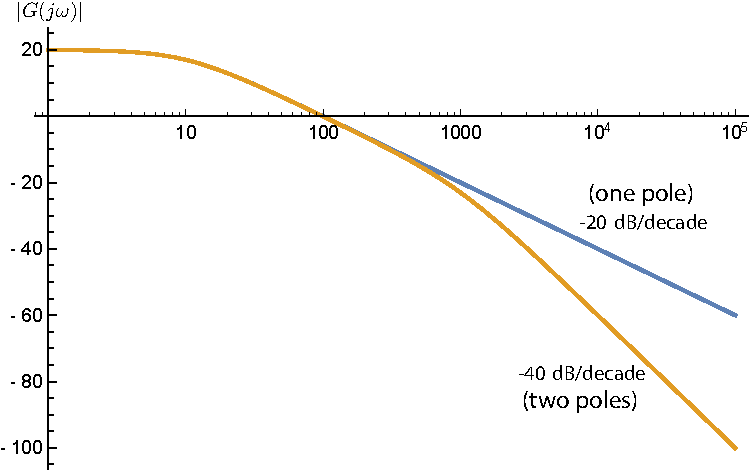
\includegraphics[width=.7\columnwidth]{mag2pole}
\caption{The magnitude response of a system with two poles drops faster, at -40 dB/dec.} \label{fig:mag2pole}
\end{figure}
%%%%%%%%%%%%%%%%%%%%%%%%%%%%%%%%%%%%%%%%%%%%
%                 FIGURE                   %
%%%%%%%%%%%%%%%%%%%%%%%%%%%%%%%%%%%%%%%%%%%%
\begin{figure}[tb]
\centering
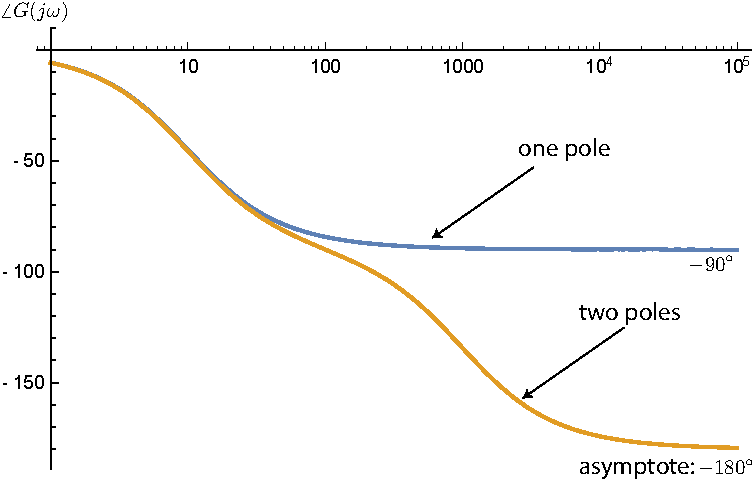
\includegraphics[width=.7\columnwidth]{phase2pole}
\caption{The phase response of a second-order transfer function has an asymptotic phase shift of 180$^\circ$.} \label{fig:phase2pole}
\end{figure}
%%%%%%%%%%%%%%%%%%%%%%%%%%%%%%%%%%%%%%%%%%%%
As we have seen, poles in the system tend to make an amplifier less stable. While a single pole cannot do harm since it has a maximum phase shift of 90$^\circ$, a second pole will bring our system to the edge of stability, shown in \emph{Figs.~\ref{fig:mag2pole} - \ref{fig:phase2pole}}.   For this reason, \textbf{non-dominant poles}\index{Poles!non-dominant} should be at a much higher frequency than the unity-gain frequency so that when the phase shift reaches 180$^\circ$, the loop gain is less than unity.
%%%%%%%%%%%%%%%%%%%%%%%%%%%%%%%%%%%%%%%%%%%%
%             SUBSECTION 17.6.3            %
%%%%%%%%%%%%%%%%%%%%%%%%%%%%%%%%%%%%%%%%%%%%
\subsection{Oscillation}
The condition $T(j\omega_x) = -1$ is in fact how we build \textbf{oscillators}\index{Oscillators}, which are inherently unstable. If the circuit has $T = -1$ at a particular frequency, then the gain at that frequency is theoretically infinite.  Any noise or disturbance can leads to a strong oscillation at this particular frequency.
\newpage
%%%%%%%%%%%%%%%%%%%%%%%%%%%%%%%%%%%%%%%%%%%%
%             SUBSECTION 17.6.4            %
%%%%%%%%%%%%%%%%%%%%%%%%%%%%%%%%%%%%%%%%%%%%
\subsection{Instability}
%%%%%%%%%%%%%%%%%%%%%%%%%%%%%%%%%%%%%%%%%%%%
%                 FIGURE                   %
%%%%%%%%%%%%%%%%%%%%%%%%%%%%%%%%%%%%%%%%%%%%
\begin{figure}[tb]
\centering
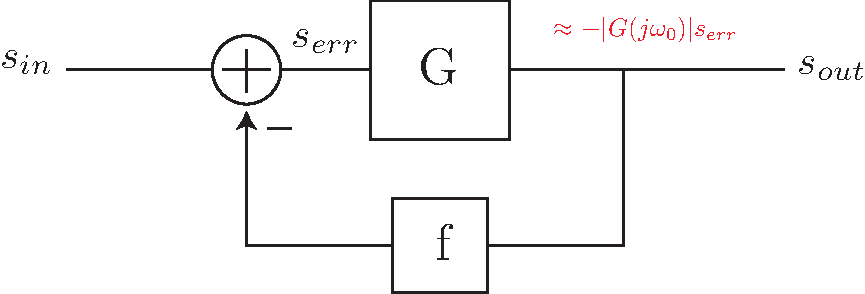
\includegraphics[scale=.7]{fbblock_phase}
\caption{A ``negative" feedback system turns into a positive feedback system at a frequency that causes phase inversion through $G$.}
\label{fig:fbblock_phase}
\end{figure}
%%%%%%%%%%%%%%%%%%%%%%%%%%%%%%%%%%%%%%%%%%%%
When the system has more poles, the phase shift can reach 180$^\circ$, as shown in \emph{Fig.~\ref{fig:fbblock_phase}}. 
This transforms the negative feedback system into a positive feedback system, which is unstable if the loop gain $|T|>1$.  

Consider the frequency $\omega_x$ that satisfies $ T(j\omega_x) = G(j{\omega _x})f =  - 1$. Since there is always noise and disturbances in the system at this frequency, this noise is regenerated and potentially can cause problems since the closed loop gain becomes infinite. The condition for stability is then to ensure that when loop gain is unity, the phase of $\angle T$ should be less than 180$^\circ$  The \textbf{phase margin}\index{Phase margin} is a measure of stability, and in practice a good design should have 60$^\circ$ phase margin or more.
%\subsection{Positive Feedback*}
%
% Positive Feedback is also useful
% We can create a comparator circuit with \textit{hysteresis}
% Also, as long as \textit{T} < 1, we can get stable gain … instead of reducing the gain (negative feedback), positive feedback enhances the gain.
% In theory we can boost the gain to any desired level simply by making T close to unity:  $T = 1-\epsilon$
% When $\epsilon$ is a very small number, the design is very risky:
%
% In practice if the gain varies over process / temperature / voltage, then the circuit can go stable and oscillate
% Positive feedback also has a narrow-banding effect (opposite of negative feedback)
